\documentclass[tikz,border=8pt]{standalone}
\usepackage{tikz}
\usetikzlibrary{arrows.meta,positioning,shapes.geometric}
\definecolor{navy}{HTML}{17365D}
\definecolor{teal}{HTML}{1B9E77}
\definecolor{orange}{HTML}{D95F02}
\definecolor{lightblue}{HTML}{EAF2F8}
\begin{document}
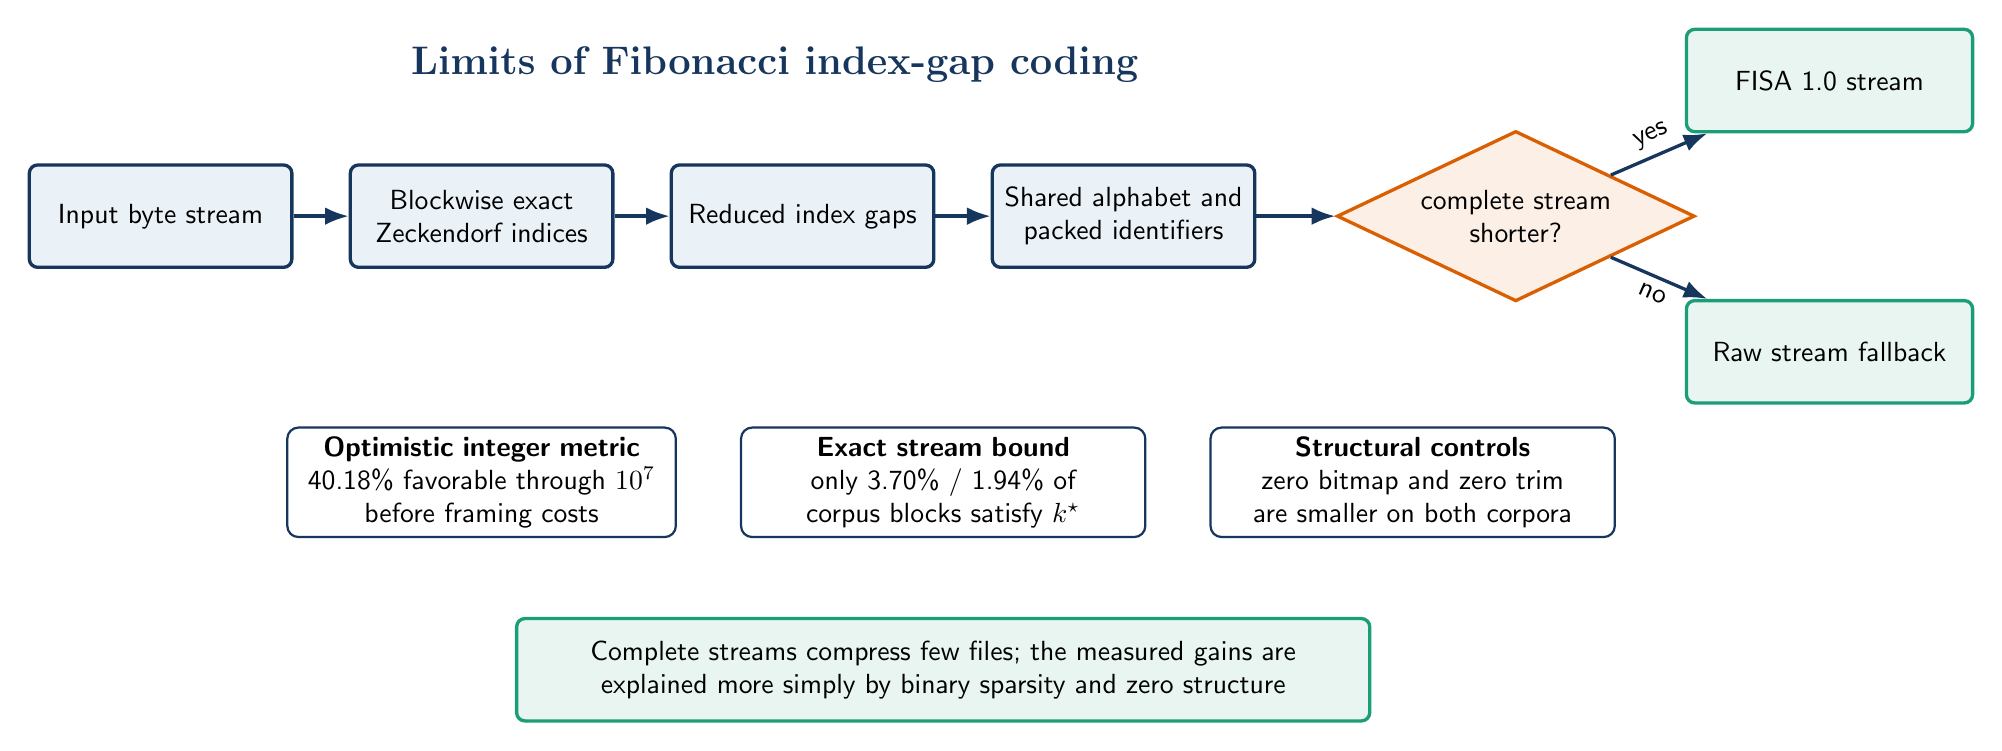
\begin{tikzpicture}[
  font=\sffamily,
  box/.style={draw=navy,rounded corners=3pt,very thick,fill=lightblue,
              minimum height=13mm,text width=31mm,align=center},
  decision/.style={draw=orange,diamond,aspect=2.1,very thick,
                   fill=orange!10,align=center},
  result/.style={draw=teal,rounded corners=3pt,very thick,fill=teal!10,
                 minimum height=13mm,text width=34mm,align=center},
  arrow/.style={-{Latex[length=3mm]},very thick,draw=navy}
]
\node[font=\bfseries\Large,text=navy] (title)
  {Limits of Fibonacci index-gap coding};
\node[box,below=9mm of title,xshift=-78mm] (bytes) {Input byte stream};
\node[box,right=7mm of bytes] (fib) {Blockwise exact\\Zeckendorf indices};
\node[box,right=7mm of fib] (gaps) {Reduced index gaps};
\node[box,right=7mm of gaps] (pack) {Shared alphabet and\\packed identifiers};
\node[decision,right=10mm of pack] (choose) {complete stream\\shorter?};
\node[result,above right=5mm and 10mm of choose] (fisa) {FISA 1.0 stream};
\node[result,below right=5mm and 10mm of choose] (raw) {Raw stream fallback};
\draw[arrow] (bytes)--(fib);
\draw[arrow] (fib)--(gaps);
\draw[arrow] (gaps)--(pack);
\draw[arrow] (pack)--(choose);
\draw[arrow] (choose)--node[above,sloped]{yes}(fisa);
\draw[arrow] (choose)--node[below,sloped]{no}(raw);

\node[draw=navy,rounded corners,thick,fill=white,below=20mm of fib,
      text width=47mm,align=center] (integer)
      {\textbf{Optimistic integer metric}\\
       40.18\% favorable through $10^7$\\before framing costs};
\node[draw=navy,rounded corners,thick,fill=white,right=8mm of integer,
      text width=49mm,align=center] (ablation)
      {\textbf{Exact stream bound}\\
       only 3.70\% / 1.94\% of\\corpus blocks satisfy $k^\star$};
\node[draw=navy,rounded corners,thick,fill=white,right=8mm of ablation,
      text width=49mm,align=center] (corpus)
      {\textbf{Structural controls}\\
       zero bitmap and zero trim\\are smaller on both corpora};
\node[result,below=10mm of ablation,text width=106mm]
  {Complete streams compress few files; the measured gains are explained more
  simply by binary sparsity and zero structure};
\end{tikzpicture}
\end{document}
